\documentclass{article}
\usepackage[margin=0.4cm,paperwidth=60cm,paperheight=32cm]{geometry}
\usepackage{tikz}
\pagestyle{empty}
\usetikzlibrary{arrows.meta,positioning}
\begin{document}\centering
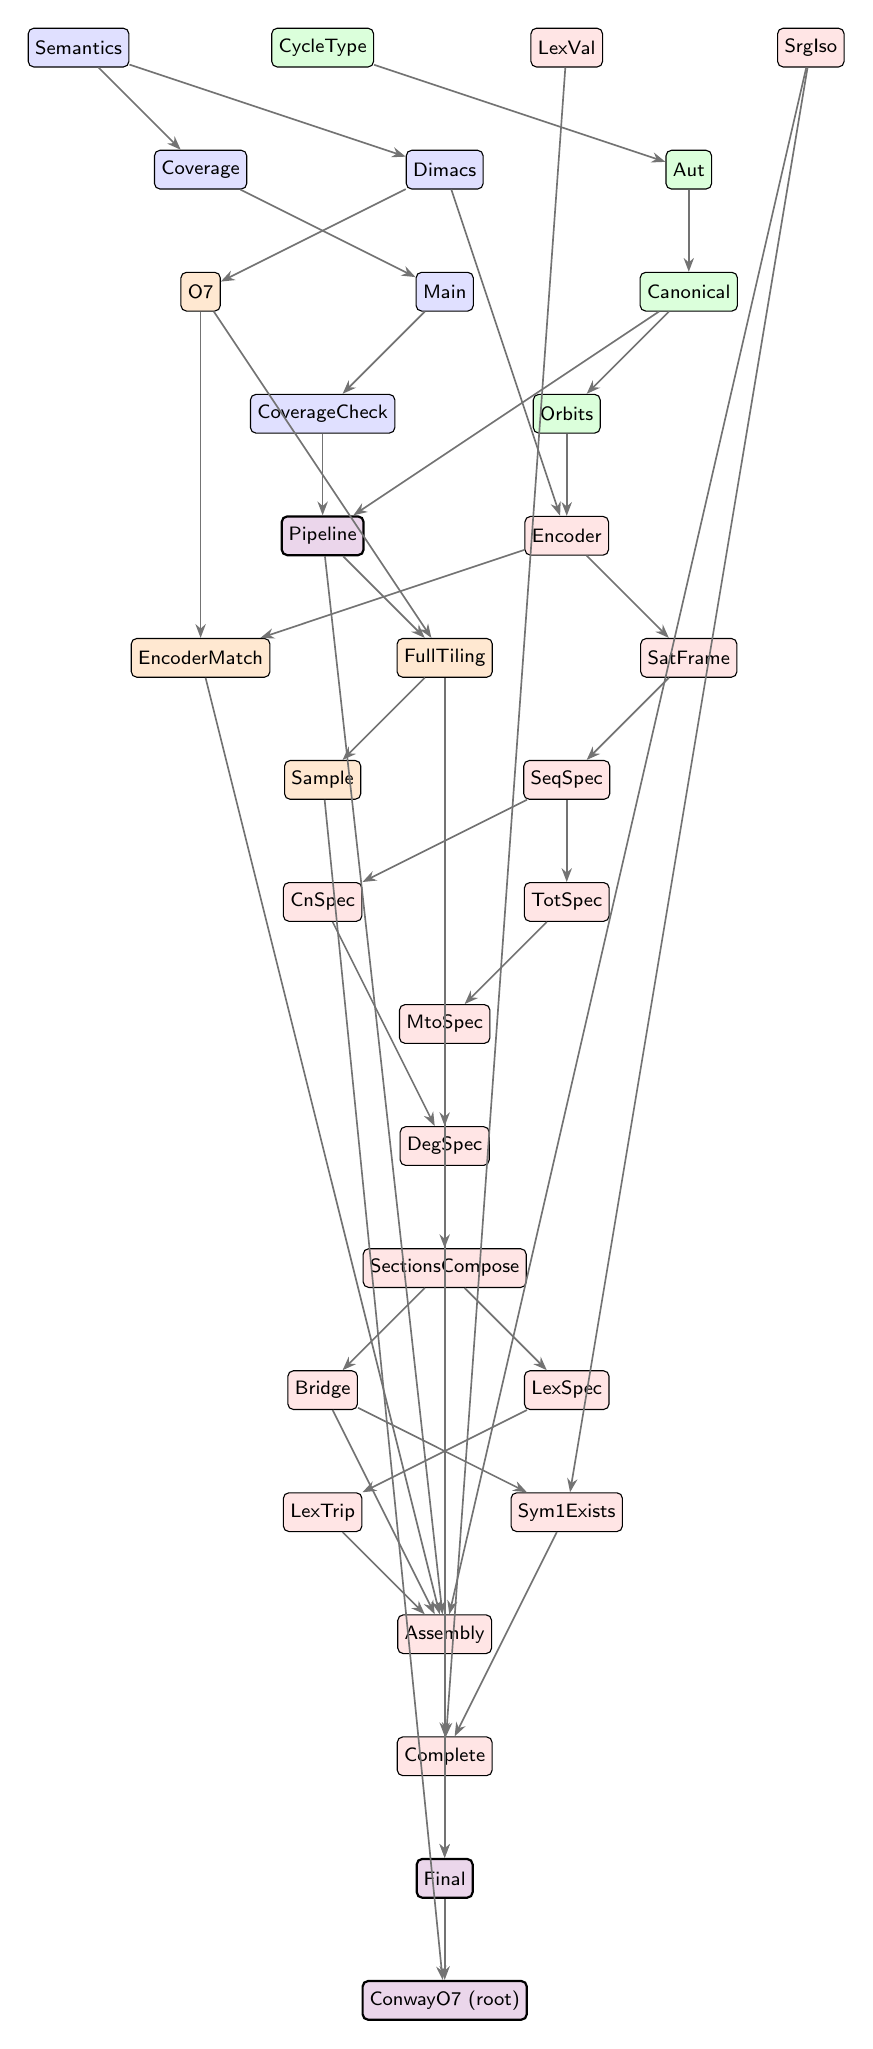
\begin{tikzpicture}[x=1cm,y=1.55cm,
  every node/.style={font=\scriptsize\sffamily,rounded corners=2pt,draw,inner sep=2.5pt,minimum height=14pt},
  l1/.style={fill=blue!12},l2/.style={fill=green!14},dat/.style={fill=orange!18},
  l45/.style={fill=red!10},end/.style={fill=violet!16,thick},
  e/.style={-{Stealth[length=5pt]},semithick,draw=black!55}]
\node[l1] (ConwayO7Semantics) at (-4.65,0) {Semantics};
\node[l2] (ConwayO7CycleType) at (-1.55,0) {CycleType};
\node[l45] (ConwayO7LexVal) at (1.55,0) {LexVal};
\node[l45] (ConwayO7SrgIso) at (4.65,0) {SrgIso};
\node[l1] (ConwayO7Coverage) at (-3.10,-1) {Coverage};
\node[l1] (ConwayO7Dimacs) at (0.00,-1) {Dimacs};
\node[l2] (ConwayO7Aut) at (3.10,-1) {Aut};
\node[dat] (ConwayO7DataO7) at (-3.10,-2) {O7};
\node[l1] (ConwayO7Main) at (0.00,-2) {Main};
\node[l2] (ConwayO7Canonical) at (3.10,-2) {Canonical};
\node[l1] (ConwayO7CoverageCheck) at (-1.55,-3) {CoverageCheck};
\node[l2] (ConwayO7Orbits) at (1.55,-3) {Orbits};
\node[end] (ConwayO7Pipeline) at (-1.55,-4) {Pipeline};
\node[l45] (ConwayO7Encoder) at (1.55,-4) {Encoder};
\node[dat] (ConwayO7DataEncoderMatch) at (-3.10,-5) {EncoderMatch};
\node[dat] (ConwayO7DataFullTiling) at (0.00,-5) {FullTiling};
\node[l45] (ConwayO7SatFrame) at (3.10,-5) {SatFrame};
\node[dat] (ConwayO7DataSample) at (-1.55,-6) {Sample};
\node[l45] (ConwayO7SeqSpec) at (1.55,-6) {SeqSpec};
\node[l45] (ConwayO7CnSpec) at (-1.55,-7) {CnSpec};
\node[l45] (ConwayO7TotSpec) at (1.55,-7) {TotSpec};
\node[l45] (ConwayO7MtoSpec) at (0.00,-8) {MtoSpec};
\node[l45] (ConwayO7DegSpec) at (0.00,-9) {DegSpec};
\node[l45] (ConwayO7SectionsCompose) at (0.00,-10) {SectionsCompose};
\node[l45] (ConwayO7Bridge) at (-1.55,-11) {Bridge};
\node[l45] (ConwayO7LexSpec) at (1.55,-11) {LexSpec};
\node[l45] (ConwayO7LexTrip) at (-1.55,-12) {LexTrip};
\node[l45] (ConwayO7Sym1Exists) at (1.55,-12) {Sym1Exists};
\node[l45] (ConwayO7Assembly) at (0.00,-13) {Assembly};
\node[l45] (ConwayO7Complete) at (0.00,-14) {Complete};
\node[end] (ConwayO7Final) at (0.00,-15) {Final};
\node[end] (ConwayO7) at (0.00,-16) {ConwayO7 (root)};
\draw[e] (ConwayO7Aut) -- (ConwayO7Canonical);
\draw[e] (ConwayO7Orbits) -- (ConwayO7Encoder);
\draw[e] (ConwayO7Dimacs) -- (ConwayO7Encoder);
\draw[e] (ConwayO7DataO7) -- (ConwayO7DataFullTiling);
\draw[e] (ConwayO7Pipeline) -- (ConwayO7DataFullTiling);
\draw[e] (ConwayO7SeqSpec) -- (ConwayO7TotSpec);
\draw[e] (ConwayO7DataSample) -- (ConwayO7);
\draw[e] (ConwayO7Final) -- (ConwayO7);
\draw[e] (ConwayO7Main) -- (ConwayO7CoverageCheck);
\draw[e] (ConwayO7DegSpec) -- (ConwayO7SectionsCompose);
\draw[e] (ConwayO7LexTrip) -- (ConwayO7Assembly);
\draw[e] (ConwayO7Bridge) -- (ConwayO7Assembly);
\draw[e] (ConwayO7Pipeline) -- (ConwayO7Assembly);
\draw[e] (ConwayO7SrgIso) -- (ConwayO7Assembly);
\draw[e] (ConwayO7DataEncoderMatch) -- (ConwayO7Assembly);
\draw[e] (ConwayO7CnSpec) -- (ConwayO7DegSpec);
\draw[e] (ConwayO7MtoSpec) -- (ConwayO7DegSpec);
\draw[e] (ConwayO7LexSpec) -- (ConwayO7LexTrip);
\draw[e] (ConwayO7Encoder) -- (ConwayO7DataEncoderMatch);
\draw[e] (ConwayO7DataO7) -- (ConwayO7DataEncoderMatch);
\draw[e] (ConwayO7Coverage) -- (ConwayO7Main);
\draw[e] (ConwayO7Semantics) -- (ConwayO7Dimacs);
\draw[e] (ConwayO7SatFrame) -- (ConwayO7SeqSpec);
\draw[e] (ConwayO7CycleType) -- (ConwayO7Aut);
\draw[e] (ConwayO7SectionsCompose) -- (ConwayO7Bridge);
\draw[e] (ConwayO7TotSpec) -- (ConwayO7MtoSpec);
\draw[e] (ConwayO7DataFullTiling) -- (ConwayO7DataSample);
\draw[e] (ConwayO7Canonical) -- (ConwayO7Orbits);
\draw[e] (ConwayO7SeqSpec) -- (ConwayO7CnSpec);
\draw[e] (ConwayO7Bridge) -- (ConwayO7Sym1Exists);
\draw[e] (ConwayO7SrgIso) -- (ConwayO7Sym1Exists);
\draw[e] (ConwayO7SectionsCompose) -- (ConwayO7LexSpec);
\draw[e] (ConwayO7Assembly) -- (ConwayO7Complete);
\draw[e] (ConwayO7Sym1Exists) -- (ConwayO7Complete);
\draw[e] (ConwayO7LexVal) -- (ConwayO7Complete);
\draw[e] (ConwayO7Encoder) -- (ConwayO7SatFrame);
\draw[e] (ConwayO7Semantics) -- (ConwayO7Coverage);
\draw[e] (ConwayO7Canonical) -- (ConwayO7Pipeline);
\draw[e] (ConwayO7CoverageCheck) -- (ConwayO7Pipeline);
\draw[e] (ConwayO7DataFullTiling) -- (ConwayO7Final);
\draw[e] (ConwayO7Complete) -- (ConwayO7Final);
\draw[e] (ConwayO7Dimacs) -- (ConwayO7DataO7);
\end{tikzpicture}
\end{document}